\documentclass[a4paper,11pt]{article}

\usepackage[utf8]{inputenc}
\usepackage[T1]{fontenc}
\usepackage[english,french]{babel}
	\frenchbsetup{SmallCapsFigTabCaptions=false}
\usepackage{indentfirst}
\usepackage[margin=1in]{geometry}
\usepackage[table,kerneldraw,dvipsnames]{xcolor}
\usepackage{pdflscape}
\usepackage{rotating}

\usepackage{csquotes}
\usepackage[natbib=true,backend=biber,style=authoryear,sort=none,sortcites=true,backref=true,backref=false,language=french,autolang=other,url=true,isbn=true,doi=true]{biblatex}
\DefineBibliographyExtras{french}{\restorecommand\mkbibnamefamily}
\addbibresource{ref.bib}
\AtBeginBibliography{\small}

\usepackage{fancyhdr}
\pagestyle{fancy}
\fancyhead{}
\fancyhead[C]{\footnotesize \itshape A. Huat / Deep Learning (2018)}

\usepackage[nopostdot,nonumberlist,toc,acronyms]{glossaries}
\renewcommand{\glossarypreamble}{\small}

\usepackage{booktabs,array,longtable,tabularx}

\usepackage{menukeys}
\usepackage[shortcuts]{extdash}
\usepackage{enumitem}
%	\setlist{itemsep=0ex}
\usepackage{multicol}
\newenvironment{colfig}{\par\medskip\noindent\minipage{\linewidth}}{\endminipage\par\medskip}

\usepackage{float}
\usepackage{graphicx}
	% Centering figures by default
	\makeatletter
	\g@addto@macro\@floatboxreset{\centering}
	\makeatother
\usepackage{here}
\usepackage{placeins}
\usepackage[labelfont=bf,justification=justified,font=small]{caption}
    \captionsetup[table]{labelsep=newline,singlelinecheck=false,name={Tableau}}
    \captionsetup[figure]{labelsep=period}
% \usepackage{floatrow}
	\floatplacement{figure}{htbp}
	\floatplacement{table}{htbp}

\usepackage[colorlinks=true,plainpages=false,breaklinks=true,allcolors=NavyBlue]{hyperref}
\usepackage{fancyref}

\usepackage{listings,listingsutf8}
	\lstset{
		breaklines=true,
		deletekeywords={},
		frame=single,
		morekeywords={pour, chaque},
		tabsize=4,
		basicstyle=\scriptsize,
		escapeinside={lx*}{*lx}
}

% Maths

\usepackage{cool}
\usepackage{upgreek}
\usepackage{upref}
\usepackage{mathtools}
\usepackage{amsmath}
\usepackage{amsfonts}
\usepackage{amsthm}
\theoremstyle{definition}
\usepackage{amssymb}
\usepackage[scaled=1.]{rsfso}
\usepackage[scaled=1.,mathscr]{urwchancal}
\usepackage{stmaryrd}

% --------------------------------------
% Macros
% --------------------------------------

\newcommand{\fnhref}[2]{\href{#1}{#2}\footnote{\url{#1}}}

\newcommand{\TODO}[1]{\textsf{\color{orange}\bfseries TODO: #1}}

\newcommand{\cad}{c'est-à-dire}
\newcommand{\Cad}{C'est-à-dire}
\newcommand{\pex}{par exemple}
\newcommand{\Pex}{Par exemple}
\newcommand{\AH}{Alexandre Huat}
\newcommand{\eg}{\textit{e.g.}}
\newcommand{\ie}{\textit{i.e.}}
\newcommand{\etc}{\textit{etc.}}
\newcommand{\etal}{\textit{et al.}}
\newcommand{\vs}{\textit{vs.}}
\newcommand{\cf}{\textit{cf.}}
\newcommand{\Cf}{\textit{Cf.}}

% Maths

% --------------------------------------
% Glossaire
% --------------------------------------

\makeglossaries

%%% Acronyms

\newacronym{eddp}{$(\epsilon, \delta)$-DP}{$(\epsilon, \delta)$--différentiellement confidentiel}

%%% Maths

% --------------------------------------
% Title
% --------------------------------------

\title{\textbf{Résumé de l'article « Differentially Private Releasing via Deep Generative Model »}}
\author{\textbf{\AH}\\Master Science des Données\\INSA Rouen Normandie\\\texttt{alexandre.huat@insa-rouen.fr}}
\date{\today}

% ======================================

\begin{document}
\maketitle
\hrule height 1.6pt

% --------------------------------------
% Body
% --------------------------------------

% \printbibliography[title=Référence] % ,heading=none
\vspace{1em}
{\small\noindent\textbf{Référence :} Zhang, Xinyang, Shouling Ji et Ting Wang (2018). « Differentially Private Releasing via Deep Generative Model ». Version 1. In : ArXiv e-prints. arXiv : \href{http://arxiv.org/abs/1801.01594}{1801.01594 [cs.CR]}.
\vspace{1em}\hrule}
\ \\

% \begin{multicols}{2}
Supposons un groupe de clients et un prestateur de services informatiques collectant et analysant leurs données (\eg\ image, texte, audio). Au cours des tâches d'analyses, le prestateur est amené à traiter des données sensibles. Afin de respecter la vie privée de ses clients, il doit trouver un moyen de traiter efficacement ces données tout en conservant leur confidentialité. C'est à cette problématique que répondent \citet{2018arXiv180101594Z}, via la méta-architecture dp-GAN\footnote{\textit{Differentially Private Generative Adversarial Network}} de l'article résumé ici.

\begin{figure}[b]
    \centering
    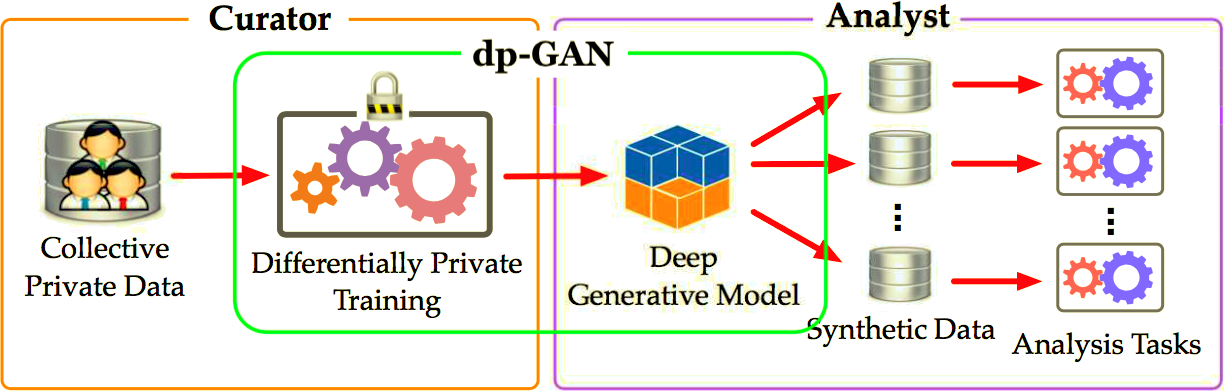
\includegraphics[width=0.67\linewidth]{dp-gan_role.png}
    \captionof{figure}{La place de dp-GAN dans la chaîne de traitement des données confidentielles. Le « \textit{curator} » est l'entité qui anonymise les données privées pour l'\textit{analyst}.}
    \label{dp-gan_role}
\end{figure}

Le rôle de dp-GAN est de générer des données synthétiques mais sémantiquement riches, \ie\ suffisamment représentatives des clients, qui pourront être utilisées sans violation de leur vie privée (\cf\ \autoref{dp-gan_role}).
En introduction, les auteurs rappellent les défis à relevér en apprentissage sous contrainte de confidentialité et présentent les apports de dp-GAN. En plus de sa capacité à générer une infinité de données, dp-GAN garantit l'anonymisation des données réelles par respect du principe de « confidentialité différentielle »\footnote{Synthétiqument, la confidentialité différentielle mesure la capacité d'un tiers à déduire des données privées des résultats d'un algorithme ; \cf\ exemple à \url{https://fr.wikipedia.org/wiki/Confidentialité_différentielle#Formalisation}.}.
% L'algorithme idéal est donc $(0, 0)$-DP, \ie\ les données sensibles sont difficilement reconstructibles via les résultats de l'algorithme qui les traite.
Pour ce faire, dp-GAN combine le réseau adverse génératif de Wisserstein amélioré (IWGAN) et des mécanismes d'anonymisation à l'état de l'art, alors optimisés pour gagner en stabilité et en scalabilité.

% \textbf{Définition}\quad{\em Soit un algorithme $\mathscr{A} \colon \mathscr{D} \to \mathscr{R}$ où $\mathscr{D}$ est une base de données et $\mathscr{R}$ un ensemble de résultats. $\mathscr{A}$ est dit \gls{eddp} si pour tous jeux de données adjacents\footnote{qui diffèrent d'un seul élémént} $d, d' \subset \mathscr{D}$ et pour tout sous-ensemble $R \subseteq \mathscr{R}$ : $\mathbb{P}(\mathscr{A}(d) \in R) \le e^\epsilon \mathbb{P}(\mathscr{A}(d') \in R) + \delta$.}

En Section 2, Zhang \etal\ font un rappel théorique sur les GAN et justifient leur utilisation d'un IWGAN par une plus grande stabilité et un plus court temps d'apprentissage que le GAN originel. Ils rappellent également la définition formelle de la confidentialité différentielle et citent des propriétés associées dont bénéficient dp-GAN.

La Section 3 de l'article présente dp-GAN dans sa version basique et fournit son algorithme d'apprentissage. Pour assurer sa confidentialité, à chaque mise-à-jour, l'algorithme bruite le gradient du discriminateur (bruitage gaussien et seuillage), qui pourrait autrement être utilisé par un pirate pour reconstruire les données privées ; cette technique est communément utilisée dans la littérature. Une preuve théorique du niveau de confidentialité différentielle atteint par l'algorithme est également apportée.

Néanmoins, cette version de dp-GAN souffre de trois inconvénients : elle génère des données de faible qualité ; elle converge moins rapidement que l'IWGAN non-confidentiel, voire diverge ; elle est rigide et n'exploite aucune ressource bonus, \eg\ des données publiques. Pour palier ces défauts, la version avancée de dp-GAN implémente : un groupage des paramètres pour un réglage fin et spécifique de leurs bruits respectifs ; un seuillage du gradient qui évolue au cours des itérations ; une initialisation des paramètres du réseau par pré-apprentissage sur les données publiques à disposition. Ces améliorations boostent la vitesse de convergence et la confidentialité de dp-GAN. La Section 4 détaille l'algorithme de  cette version avancée.

S'en suit un rapport d'expériences sur trois bases célèbres et \textit{open source}, étendues à quatre : \fnhref{http://yann.lecun.com/exdb/mnist/}{MNIST}, \fnhref{http://mmlab.ie.cuhk.edu.hk/projects/CelebA.html}{CelebA} et \fnhref{http://lsun.cs.princeton.edu/2015.html}{LSUN}, LSUN étant divisée en deux bases, l'une labellisée (LSUN-L) et l'autre non-labellisée (LSUN-U). Les expériences sont réalisées avec TensorFlow mais le code n'est pas partagé par ses auteurs ; les paramètres testés sont cependant renseignés. La Section 5 propose ainsi une évaluation qualitative et quantitative des performances du système. De mon point de vue, les images générées par dp-GAN, quelque soit la base, sont assez vraisemblables ; MNIST en particulier est très bien representée mais il subsiste un léger bruit de pixels isolés sur chaque image. L'évaluation quantitative, quant à elle, repose sur deux métriques statistiques. D'une part, le score \textit{Inception}, pour les données labellisées, défini par :
\begin{equation}
    \label{incep}
    \mathrm{Inc}(G) = \exp(\mathbb{E}_{x \sim G(z)}[\mathrm{KL}(\mathbb{P}(y \mid x)\,\Vert\, \mathbb{P}(y))])
\end{equation}
où G est un générateur.
D'autre part, le score de Jensen-Schannon, pour les données non-labellisées, défini par :
\begin{equation}
    \label{jens}
    \mathrm{JS}(G) = \frac{1}{2} \mathrm{KL}(\mathbb{P}(y \mid x)\,\Vert\,\mathscr{B}_p)
    + \frac{1}{2} \mathrm{KL}(\mathscr{B}_p\,\Vert\,\mathbb{P}(y \mid x))
\end{equation}
où $\mathscr{B}_p$ est une loi de Bernouilli de paramètre $p=\frac{1}{2}$.

% \end{multicols}
\end{document}
